\documentclass[a4paper,12pt]{article}

\usepackage{amsmath,amssymb,amsthm,tikz}
\usepackage{fancyvrb}
\usetikzlibrary{calc,arrows.meta}
\usepackage[margin=20mm]{geometry}
\usepackage{multicol}

\setlength{\parindent}{0pt}
\setlength{\columnsep}{1cm}


\begin{document}\thispagestyle{empty}

\twocolumn

\begin{center}
{\Large Sample Problems: Stacks and Queues}\\
{\em Published on 2020-10-19}
\end{center}

Warm-up exercises offered before the midterm.

\vspace{10pt}
{\bf \large (1) Stack Implementation.} 

Stack is implemented as an array. In our case the array has size $n = 5$. 
Stack contains integer numbers; initially the array has 
the following content.

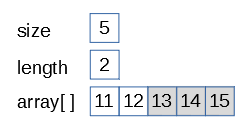
\includegraphics[width=2.2in]{sample-stacks-queues/stack-structure.png}

Stack has the physical representation with $\mathtt{length}=2$
(the number of elements in the stack), $\mathtt{size}=5$ (maximal number of elements
contained in the stack). We have the following fragment:

\begin{center}
\begin{minipage}{.8\columnwidth}
\begin{Verbatim}[frame=single,numbers=left]
pop();
push(21);
push(22);
pop();
push(23);
push(24);
pop();
push(25);
\end{Verbatim}
\end{minipage}
\end{center}


Draw the state of the array after every command. 
(Every {\tt push(elt)} command assigns a new element into the element {\tt array[length]}, 
then increments {\tt length} by $1$.
The command {\tt pop()} does not modify the array, but decreases {\tt length} by $1$. 

If the command cannot be executed ({\tt pop()} on an empty stack; {\tt push(elt)} on a full stack), 
then the stack structure does not change at all (either {\tt array} or {\tt length}). 
To help imagine the state of this stack, you can shade those cells that do not belong to the array.








\vspace{20pt}
{\bf \large (2) Queue Implementation.}

A queue is implemented as an array with {\tt size} elements; it has two
extra variables {\tt front} (pointer to the first element) and {\tt length} 
(the current number of elements in the queue). Current state is shown in the figure:

\begin{center}
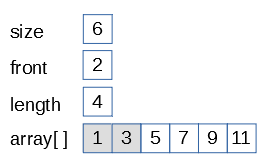
\includegraphics[width=2.3in]{sample-stacks-queues/queue-structure.png}
\end{center}



Enumeration of array elements starts with $0$. The array is filled in a circular
fashion. The command {\tt enqueue(elt)} inserts a new element at 
$$(\mathtt{front}+\mathtt{length})\;\mbox{mod}\;\mathtt{size},$$
where "mod" means the remainder when dividing by {\tt size}. It also increments the 
{\tt length} element.\\
The command {\tt dequeue()} does not change anything in the array, it increments
{\tt front} by $1$ and decreases {\tt length} by $1$. Thus the queue becomes shorter by $1$. 

\begin{center}
\begin{minipage}{.8\columnwidth}
\begin{Verbatim}[frame=single,numbers=left]
dequeue(); 
enqueue(21);
dequeue(); 
enqueue(22);
enqueue(23);
enqueue(24);
dequeue();
\end{Verbatim}
\end{minipage}
\end{center}

Show the state of the array after every command \textendash{} {\tt array,length, front} 
variables after every line. (Shade the unused cells.)


\vspace{20pt}
{\em Note.} In the actual midterm the starting state may 
be different, other command sequence (may also include conditionals
and/or loops), it may be parametrized by the digits of your Student ID
or by numbers computed from these digits. 




\newpage

{\bf \large Solutions}


\vspace{10pt}
{\bf (1) Stack Implementation:}


\begin{center}
\begin{minipage}{.8\columnwidth}
\begin{Verbatim}[frame=single,numbers=left]
pop();
push(21);
push(22);
pop();
push(23);
push(24);
pop();
push(25);
\end{Verbatim}
\end{minipage}
\end{center}

\begin{center}
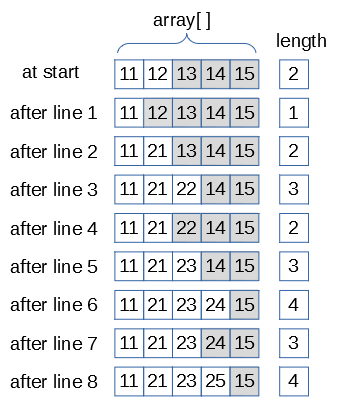
\includegraphics[width=2.7in]{sample-stacks-queues/stack-solution.png}
\end{center}

\vspace{20pt}
{\bf (2) Queue Implementation:}


\begin{center}
\begin{minipage}{.8\columnwidth}
\begin{Verbatim}[frame=single,numbers=left]
dequeue(); 
enqueue(21);
dequeue(); 
enqueue(22);
enqueue(23);
enqueue(24);
dequeue();
\end{Verbatim}
\end{minipage}
\end{center}

\begin{center}
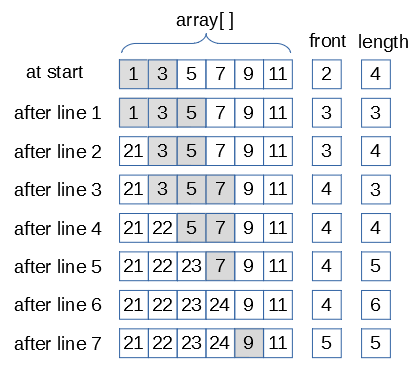
\includegraphics[width=3in]{sample-stacks-queues/queue-solution.png}
\end{center}


\end{document}



